\documentclass[a4paper,10pt]{article}
\usepackage[utf8]{inputenc}
\usepackage{float}
\usepackage{pgfplotstable}
\usepackage{amsfonts}
\usepackage{listings}
\usepackage[parfill]{parskip}
\usepackage{amsmath}
\usepackage{graphicx}
\usepackage{adjustbox}
\usepackage{enumitem}
\usepackage{setspace}
\usepackage{float}
\onehalfspacing
\usepackage[margin=0.8in]{geometry}

% \float­place­ment{fig­ure}{H}
\pgfplotsset{compat=1.13}


\pgfplotstableread[col sep=comma]{
Dataset,DT,DT-RI,TB,RF,F-RI,RF-RI
Titanic,0.78,0.79,0.77,0.75,0.78,0.74
Pima,0.75,0.76,0.69,0.65,0.71,0.63
Banknote,0.93,0.9,0.87,0.86,0.88,0.83
}\mytable

\pgfplotstableread[col sep=comma]{
Dataset,DT,DT-RI,TB,RF,F-RI,RF-RI
Titanic,0.19,0.14,1,0.45,0.99,0.48
Pima,0.2,0.19,0.77,0.26,1,0.28
Banknote,0.17,0.18,0.63,0.54,1,0.56
}\mytimes


\definecolor{blueaccent}{RGB}{0,150,214}
\definecolor{greenaccent}{RGB}{0,139,43}
\definecolor{purpleaccent}{RGB}{130,41,128}
\definecolor{orangeaccent}{RGB}{240,83,50}
\definecolor{redaccent}{RGB}{130,10,10}
\definecolor{yellowaccent}{RGB}{250,220,100}
\definecolor{blackaccent}{RGB}{100,100,100}


\newcommand{\pagetitle}[1]{{\Large \textbf{#1}}\vspace{1.5em}}
\begin{document}

%----------------------------------------------------------------------------------------
%	TITLE PAGE
%----------------------------------------------------------------------------------------
\begin{titlepage}
  \newcommand{\HRule}{\rule{\linewidth}{0.5mm}}

  \center % Center everything on the page
  %----------------------------------------------------------------------------------------
  %	HEADING SECTIONS
  %----------------------------------------------------------------------------------------

  % LOGOS UPC I FIB
  \begin{minipage}[c]{0.4\linewidth}
    \hspace{0.12\linewidth}%
    
\includegraphics[keepaspectratio, width=0.76\linewidth]{images/UPC.jpg}
  \end{minipage}%
  \hspace{0.1\linewidth}%
  \begin{minipage}[c]{0.4\linewidth}
    
\includegraphics[keepaspectratio, width=\linewidth]{images/FIB.jpg}
  \end{minipage}

  \vspace{4em}

  %\textsc{\Large Universitat Polit\`ecnica de Catalunya}\\[2cm] % Name of your university/college
  \textsc{\LARGE Algorithmics for Data Mining}\\[0.5cm] % Major heading such as course name

  %----------------------------------------------------------------------------------------
  %	TITLE SECTION
  %----------------------------------------------------------------------------------------
  \HRule \\[0.4cm]
         { \huge \bfseries CART and Random Forests in Python 3.5}\\[0.4cm] % Title of your document
         \HRule \\[7.5cm]
         
         %----------------------------------------------------------------------------------------
         %	AUTHOR SECTION
         %----------------------------------------------------------------------------------------
         \begin{minipage}[t]{0.55\textwidth}
           \begin{flushleft}% \large
             \emph{Authors:}\\
             Pol Alvarez Vecino \\
           \end{flushleft}
         \end{minipage}
         ~
         \begin{minipage}[t]{0.4\textwidth}
           \begin{flushright}% \large
             \emph{Professor:} \\
             Jose Luis Balcázar Navarro
           \end{flushright}
         \end{minipage}\\[1.5cm]

         %----------------------------------------------------------------------------------------
         %	DATE SECTION
         %----------------------------------------------------------------------------------------
         {April 27th 2017, Barcelona}\\[3cm] % Date, change the \today to a set date if you want to be precise
         \vfill % Fill the rest of the page with whitespace

\end{titlepage}
\tableofcontents

\newpage

\begin{abstract}

This project explores diverse classifiers based on classification tree, implements some of them, and discusses some improvements and issues for each technique. The basic implemented methods are the classic C4.5 for creating classification trees and its extension with randomized input technique. Upon this, tree bagging was coded as a first step for the posterior random forest implementation. 

\end{abstract}





\section{Introduction}

The project's goal is to explore and implement classification and regression trees and use them as basic block to implement the ensemble method random forest. First, I developed a basic functional implementation of a decision tree using the Gini index to make the splits. This first naive approach was then improved adding better pruning, performance optimizations, creating a class for the decision tree, and using \textit{information entropy} as rule to decide the splits. The result was the C4.5 \cite{Quinlan1993} algorithm implementation and a robust tree class upon which the more complex techniques and methods were built. 

The first improvement was the so called random input technique in which, instead of choosing always the best split for each node, one out of the best 20 is chosen minimizing the variability of the model. Another method to minimize the variance of the model is the bootstrap aggregating or bagging method with replacement \cite{Breiman2001} in which we train various trees with a random subset of the dataset with repetitions. With this variant, we use the class with maximum occurences of a class over all the trained trees to make a prediction for an element. 

Next implementation was the random forest with random input selection. The base is the same as bagging: accumulating multiple trees. However, here we consider just a subset of all the features in each split. This subset is randomly selected every time. The number of features selected in our tests was one of the usually agreed values: $\sqrt{\# attributes}$.

For this project, I decided to use libsvm format through all the implementations as input. However, the trees use a custom representation more according to the pythonic way enhancing the programming and code clarity. This representation is a list where each element is the value of an attribute and the last one is the target. Parameter names are abstracted when mapping the dataset so we can consistently work only with variables indices making the tree splits easier to code and understand.

\section{Preliminar considerations}

All the implemented versions of the trees are designed for numerical ordinal data. It assumes that all attributes values are numbers and the order among them matters (such as age, income, etc...). However, the implementations can deal out-of-the-box with 2-valued categorical variables because order among strings in python is defined (no need to cast to integer) and then the splits tested will be one value against the other. 

For testing implementations I used the Titanic survival dataset. It is not correct to do so because even if two of the three attributes are have only 2 values (male vs female, adult vs child) and the third variable is enconded in such a way that the string order makes sense (1st $>$ 2nd $>$ 3rd $>$ Crew), the ordering could be irrelevant to the classification. However, I used it nonetheless because we already knew that first class has greater chances than crew and it is a quite explanatory example.

Another consideration to be made is that variables have not been thresholded, for each possible value an split is computed. In attributes with arbitrary precision this can lead to the evaluation of an split for each element and for each variable with a cost of $O(n*m)$ (being n the number of elements and m the number of attributes) which is can lead to extremely high training times for relatively big datasets making the method impractical. 

To solve this, the trees should evaluate the values in ranges (if the attribute is a probability it could be, for example, divided into a evaluation split every 0.1). However, choosing the correct thresholds adds another layer of complexity to the problems and the focus of this work was to review the techniques not to fine-tune each hyperparameter of the tree to get the maximum accuracy possible. Because of that, no thresholding was performed and all the techniques are reviewed from a theoretical point of view without actually comparing performance among them.

\section{Functional Decision Tree}

Associated files:
\begin{description}
 \item [· functional\_decision\_tree.py,] implements a functional version of a decision tree.
\end{description}

This first implementation uses Gini index to construct a tree in a functional fashion (i.e. it only uses a dictionary to represent the tree, not a dedicated class). The growth of the the tree can be controlled through two parameters: minimum elements per node and maximum depth of the tree. This version tried all possible splits at each node and selected the best according to the Gini index. For binary targets the "Gini measure of impurity" of a node $t$ is

\[G(t) = 1 - p(t)^2 - (1-p(t))^2\]

where $p(t)$ is the relative frequency of one of the classes. Worth noting is that $p(t)$ can be weighted.

This first model has many issues because it is a simple implementation. First, if the Gini index of a group is already perfect (0) then all his descendants will have perfect Gini score also but this version will keep splitting the groups until the max depth or min number of elements per leaf is reached. Another issue is that the exploration is not prunned. This means that if two elements have the same value in a parameter the Gini index will be computed twice slowing the evaluation. 


\section{C4.5}

Associated files:
\begin{description}
 \item [· decision\_tree.py,] contains class implementing a decision tree built with C4.5 algorithm
\end{description}

C4.5 implementation uses information entropy instead of the Gini index to choose the splits. The improvement generated by splitting a node $P$ into left $L$ and right $R$ nodes is

\[ I(P) = G(P) - q*G(L) - (1-q)*(G(R) \]

where $q$ is ratio of instances going left to the total and $G(*)$ is the Gini index of a node. Again, $q$ can be weighted.

Though not being reported in the results, the change from Gini to entropy information yielded a 9\% accuracy increase in the Titanic database. Other purity measure such as twoing, ordered twoing or symmetric Gini were considered but not implemented.

This version also has better prunning based in the entropy index: if the next split does not has a positive valued entropy score the recursion is stopped. On the other hand, if the split yields a small (but irrelevant) improvement it will be a candidate so the amount of information considered relevant enough to split should be controlled. Two possible options that come to mind are to threshold the minimum required value or to compare the actual split value with its parent value (and stop the exploration if difference is small enough).

The splits exploration is also improved, now each attribute-value explored is saved into a set of already explored pairs avoiding testing them more than once per node.

This implementation is encapsulated inside a class which allowed a hassle-free string representation. Listing 1 shows the output of printing a tree and Figure \ref{fig:tree} is the previous tree in a more visual representation for the Titanic dataset. 

\begin{lstlisting}[language=bash,caption={String representation of a decision tree with a maximum of 2 and at least one element per node for the Titanic dataset. As expected, the most important factor is sex. The next two are belonging to 3rd class vs. the rest and age (child vs. adults)}]
- Decision Tree
[Attr:Sex - Val:Male]: Score=0.091
 [Attr:Class - Val:3rd]: Score=0.092
  [Yes] (0.93): ['Child', 'Female', '2nd']
  [Yes] (0.5): ['Child', 'Female', 'Crew']
 [Attr:Age - Val:Child]: Score=0.004
  [No] (0.8): ['Adult', 'Male', 'Crew']
  [No] (0.55): ['Child', 'Male', '3rd']
Training time: 0.05
Testing time: 0.01
Total accuracy: 0.78
\end{lstlisting}

\begin{figure}[htpb]
\centering
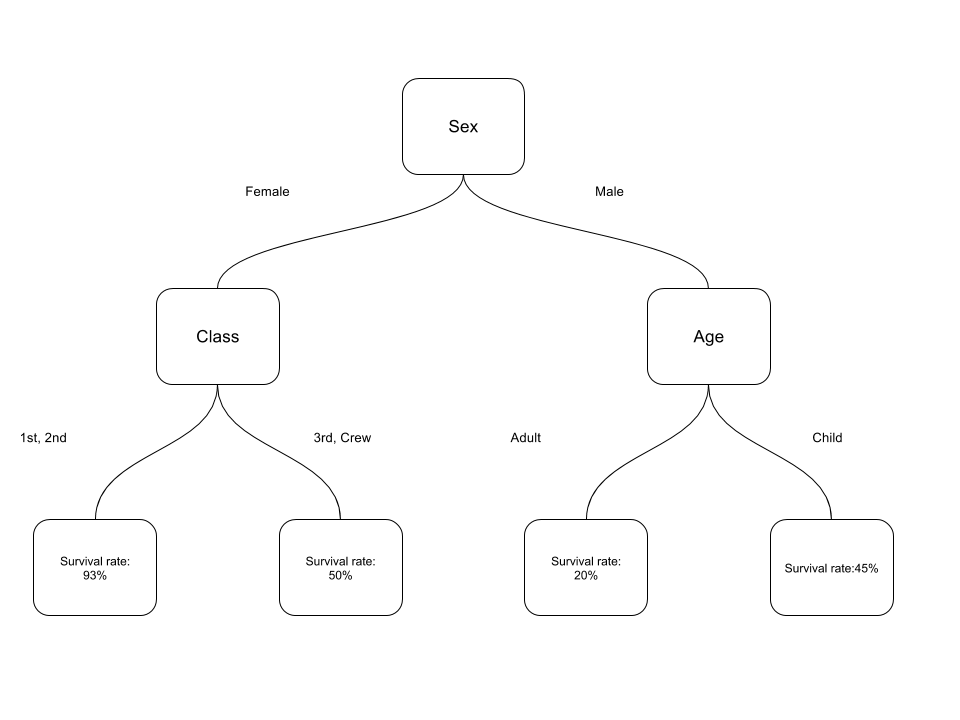
\includegraphics[keepaspectratio, width=15cm]{images/tree.png}
\caption{Visual representation of tree from Listing 1}
\label{fig:tree}
\end{figure} 

\section{Randomized input}

Associated files:
\begin{description}
 \item [· decision\_tree.py,] contains class implementing a decision tree built with C4.5 algorithm
\end{description}

The random input technique is used to decrease the effect of noise in the data. Instead of selecting always the best split, the algorithm selects randomly one out of the 20 best. The tests performed did not show any significant improvement with respect to the basic exploration (for two datasets 1\% improvement for the other 2\% decrease). However, in order to benefit from this technique, datasets should have a significant number of attributes because otherwise only 1 or 2 attributes are explored biasing a lot the predictor if we use shallow trees (especially when training a single tree instead of a forest).

\section{Forests}

This section describes the four methods were multiple trees are trained to produce a single classifier. The methods are:

\begin{itemize}
 \item Bootstrap aggregating or Tree bagging
 \item Random forest
 \item Forest with random input
 \item Random forest with random input
\end{itemize}

The four methods are orchestrated from the same file, random\_forest.py, because the basic structure is the same. For the bagging version, before the training the sampling is performed. For the last three, the basic decision tree implementation was parametrized to support all methods. For random forests, before testing the splits, a subset of features is removed from the exploration. The forest with random input just trains a set of trees (with best out of 20 selected as split). Last version uses all the randomization techniques (except bagging).

The last two methods do not have an specific section because they are combinations of the random input and random feature selection. The methods that do not use bagging (last three) were also tested with bagging with no significant variation in the testing setup so the results were not reported to avoid cluttering the tables and figures with too much information.

To speed up the forest training time, individual forests are trained in parallel. Specifically, the algorithm uses twice the number of cores available as number of simultaneosly trained trees (oversubscribing the computer threads by a factor of 2).



\subsection{Tree Bagging}

Associated files:
\begin{description}
 \item [· random\_forests.py,] orchestrator class that trains tree in parallel and handles prediction
 \item [· decision\_tree.py,] contains class implementing a decision tree built with C4.5 algorithm
\end{description}

Bootstrap aggregating or bagging technique is sampling technique used to reduce the variance of the classifier and increase tolerance to noise in the input data. When used, instead of training one tree we use a set of trees. 

This sampling has been implemented in the random forest file, specifically, each tree training is responsible of bagging the sample that will be used for the decision tree construction. The sources found, suggest using the same number of elements to bag (i.e. number of elements to be sample) and tree to be trained. This is highly impractical for the extreme cases (use 4 elements to train 4 trees, or use 10000 elements to train 10000 trees) because it uses too few elements or the training time becomes too high. Instead, for the tests we draw the same number of elements as the input dataset, and just set the number of trees to be trained. This effect of this is to weight some instances (because they can be repeated).

\subsection{Random forest}

Associated files:
\begin{description}
 \item [· random\_forests.py,] orchestrator class that trains tree in parallel and handles prediction
 \item [· decision\_tree.py,] contains class implementing a decision tree built with C4.5 algorithm
\end{description}

The random forest technique is based in exploring just a subset of all the attributes. For each split, we get $k$ attributes and decide the split based on only this ones. The number used for classification is normally $\sqrt{\# attributes}$ and $p/3$ for regression. Randomly subsetting reduces the variance of the models and greatly decreases the execution time (see \ref{sec:results}).


\section{Experiments}
\label{sec:experiments}

Associated files:
\begin{description}
 \item [· run\_predictors.py,] file orchestrating all the tests execution.
\end{description}

The experiments performed used Python 3.5. To run them just issue the Listing 2. commands inside the folder \textit{"./classifiers/src"}.

\begin{lstlisting}[language=bash,caption={Execution commands to reproduce reported results}]
python3 run_predictors.py
\end{lstlisting}

This will run the 3 datasets with a the following parametrizations: 

\begin{table}[h]
    \centering
    \begin{tabular}{|c|c|c|c|}
        \hline
        \textbf{Method}   & \textbf{Number of Trees}     & \textbf{Max. Depth} & \textbf{Min. per Node} \\ \hline
	  Decision Tree & - & 5 & 1 \\ \hline
	  Decision Tree with Random Input & - & 5 & 1 \\ \hline
	  Tree bagging & 32 & 5 & 1 \\ \hline
	  Random Forest & 32 & 5 & 1 \\ \hline
	  Forest with Random Input & 32 & 5 & 1 \\ \hline
	  Random Forest with Random Input & 32 & 5 & 1 \\ \hline
    \end{tabular}	
    \caption{Parametrizations for each method used.}
\end{table}



\subsection{Datasets}
\label{subsec:datasets}

The datasets used are the PIMA Indians diabetes \footnote{https://archive.ics.uci.edu/ml/datasets/Pima+Indians+Diabetes}, the banknote authentication  \footnote{http://archive.ics.uci.edu/ml/datasets/banknote+authentication}, and the Titanic (just for reference). All the datasets are formated following libsvm format.

Datasets files and classification objective:

\begin{description}
 \item [· banknote.txt,] predict if a banknote is fake depending on visual features.
 \item [· pimaTr.txt,] predict if an individual has diabetes
 \item [· titanicTr.txt,] surival to the Titanic accident.
\end{description}

\subsection{Cross-validation}
\label{subsec:validation}

The validation method used in the experiments is 10-fold and 10 iterations cross-validation (10x10CV). For each method and dataset, data is shuffled and 10 cross-validation is performed. This is repeated 10 times, reshuffling data every time. The final model accuracy is the average of all partial ones.

For methods using bagging, out-of-bag (OOB) measure should be used because with it we could use the whole dataset (instead of doing CV) as the bagging already handles the training/testing division. 

\section{Results}
\label{sec:results}
The results are only illustrative to draw some observations and discuss the methods because every method should be tuned to get the best results which, in turn, affect how we produce those results (CV vs. OOB). Forests, in general, will suffer the most because the datasets used have little noise and the lack of optimization makes them impractically slow (further difficulting the tuning of the hyperparameters).

\begin{figure}[H]
\begin{tikzpicture}
  \begin{axis}[
    width=0.8*\linewidth,
    ybar,
    bar width=7.5pt,
    ymin=0.5,
    enlarge x limits={abs=55pt},
    legend style={draw=none,at={(0.5,-0.15)},
    anchor=north,legend columns=-1},
    xlabel={Datasets},
    ylabel={Accuracy},
    symbolic x coords={Titanic, Pima, Banknote},
    xtick=data,
    cycle list={blueaccent,greenaccent,purpleaccent,redaccent,yellowaccent, blackaccent}
  ]
    \pgfplotsinvokeforeach{DT, DT-RI, TB, RF, F-RI, RF-RI}{
      \addplot+[draw=none,fill,] table[x=Dataset,y=#1]{\mytable};
      \addlegendentry{#1}
    }
\end{axis}
\end{tikzpicture}
\caption{Accuracy for each method: Decision Tree (DT), Decision Tree with Random Input (DT-RI), Tree bagging (TB), Random Forest (RF), Forest with Random Input (F-RI), Random Forest with Random Input (RF-RI). Probably, single trees methods work always best because of the inability to explore a significant amount of trees for ensemble methods and because datasets do not have a lot of noise.}
\label{fig:accuracy}
\end{figure}
\begin{figure}[H]
\begin{tikzpicture}
  \begin{axis}[
    width=0.8*\linewidth,
    ybar,
    bar width=7.5pt,
    ymin=0,
    enlarge x limits={abs=55pt},
    legend style={draw=none,at={(0.5,-0.15)},
    anchor=north,legend columns=-1},
    xlabel={Datasets},
    ylabel={Execution time (normalized)},
    symbolic x coords={Titanic, Pima, Banknote},
    xtick=data,
    cycle list={blueaccent,greenaccent,purpleaccent,redaccent,yellowaccent, blackaccent}
  ]
    \pgfplotsinvokeforeach{DT, DT-RI, TB, RF, F-RI, RF-RI}{
      \addplot+[draw=none,fill,] table[x=Dataset,y=#1]{\mytimes};
      \addlegendentry{#1}
    }
\end{axis}
\end{tikzpicture}
\caption{Normalized execution times for each method. Times have been normalized in a per-dataset basis in order to fit them all in a single figure, Table \ref{tab:times} shows the actual unmodified times. Methods that use random features exploration (RF, RF-RI) show a notable performance increase with respect to the ones that do not (TB, F-RI). Selecting the best out of 20 instead of the best split shows a performance increase in two of the datasets. This can only be caused by the fact that a random selection led to a faster convergence. It is worth noting that ensemble methods can not be directly compared to the single trees because forests are trained in parallel (with twice the number of the computer cores trees trained simultaneosly).}
\label{fig:times}
\end{figure}


\begin{table}[H]
    \centering
    \begin{tabular}{|c|c|c|c|c|c|c|}
        \hline
	  Dataset & DT & DT-RI & TB & RF & F-RI & RF-RI \\ \hline
	  Titanic & 0.32 & 0.23 & 1.68 & 0.76 & 1.66 & 0.8 \\ \hline
	  Pima & 8.04 & 7.69 & 30.76 & 10.6 & 40.2 & 11.1 \\ \hline
	  Banknote & 36.09 & 39.01 & 135.13 & 114.51 & 212.21 & 119.45 \\ \hline
    \end{tabular}	
    \caption{Training times for each dataset and method explored in seconds.
    \label{tab:times}
}
\end{table}


The results of Figure \ref{fig:accuracy} show that single tree methods work best in our scenarios. The reasons are probably that datasets do not have a lot of noise and training a significant number of trees for the forest methods is impractical due to their exponentially increasing execution time. We see that Random Forests based methods (RF and RF-RI) are the worst. Exploring just a random subset of the attributes with these datasets (which contain a small number of attributes) limits the exploration to only 1 parameter and we set the depth to only 5 levels thus, using only 1 attribute, biases a lot the exploration. 

However, random p-features exploring yields times three times lower (a 3x speed up) which suggests that finely tuned this methods could retain the same quality with less training time.


\section{Conclusions and Future Work}

The resulting implementation in Python is clean and understandable. However, the lack of typing made the coding a bit more cumbersome to debug the structures of the trees and forests. I tried the type annotations introduced in Python 3.5 in order to make the code clearer but they are still far from being a panacea. First, they cannot be used when default values are specified for a parameter; second, Python does not perform any check out of the box for them; and finally, in order to specify comple structures as type annotation (such as the split and terminal nodes) requires to create an specific empty interface (in this case it would be a "node" interface).

The testing results, albeit not complete nor fine-tuned, show that using random input improves the performance and decreases training times in some cases, which is quite significative because these are small datasets with not much noise where the impact of randomizing is smaller. For the ensemble methods, subsetting the feature exploration yields huge training time improvements at the cost of decreasing the accuracy an average 2\%. Finally, combining both the randomization techniques only results in worse accuracy and higher execution times in the tested datasets.

As future work, it would be interesting to correct the issues pointed out throughout all the document in order to be able to benchmark correctly the assess the performance and accuracy of each of the methods. This would include thresholding numerical values, add support for categorical variables (one vs. all splits), modify the minimum value for convergence of the entropy information, and use oob errors to prune the tree and evaluate splits. 

Another interesting comparison would be between AdaBoost ensemble method with decision stumps and a well calibrated random forest. 

% With respect to TANaiveBayes, the method had good results although not significative enough (could be the reason why they are not one of the most applied methods). As future work we could try to manually construct the dependencies tree (or at least tweak it) with the help of an expert of the data and see if that yields better results. 
% 
% Finally, we have extended the confusion matrix, accuracy, and sensitivity for muticlass problems and decided how to average and report them when dealing with 10x10CV. Despite that, we have seen that the gathered results, even if useful, did not provide enough information to clear picture of the performance. It would be interesting to complement these numerical results with ROC curves and more detailed metrics (were averaging does not hide or bias the regular values). 

\bibliography{bibliography} 
\bibliographystyle{ieeetr}

\end{document}
